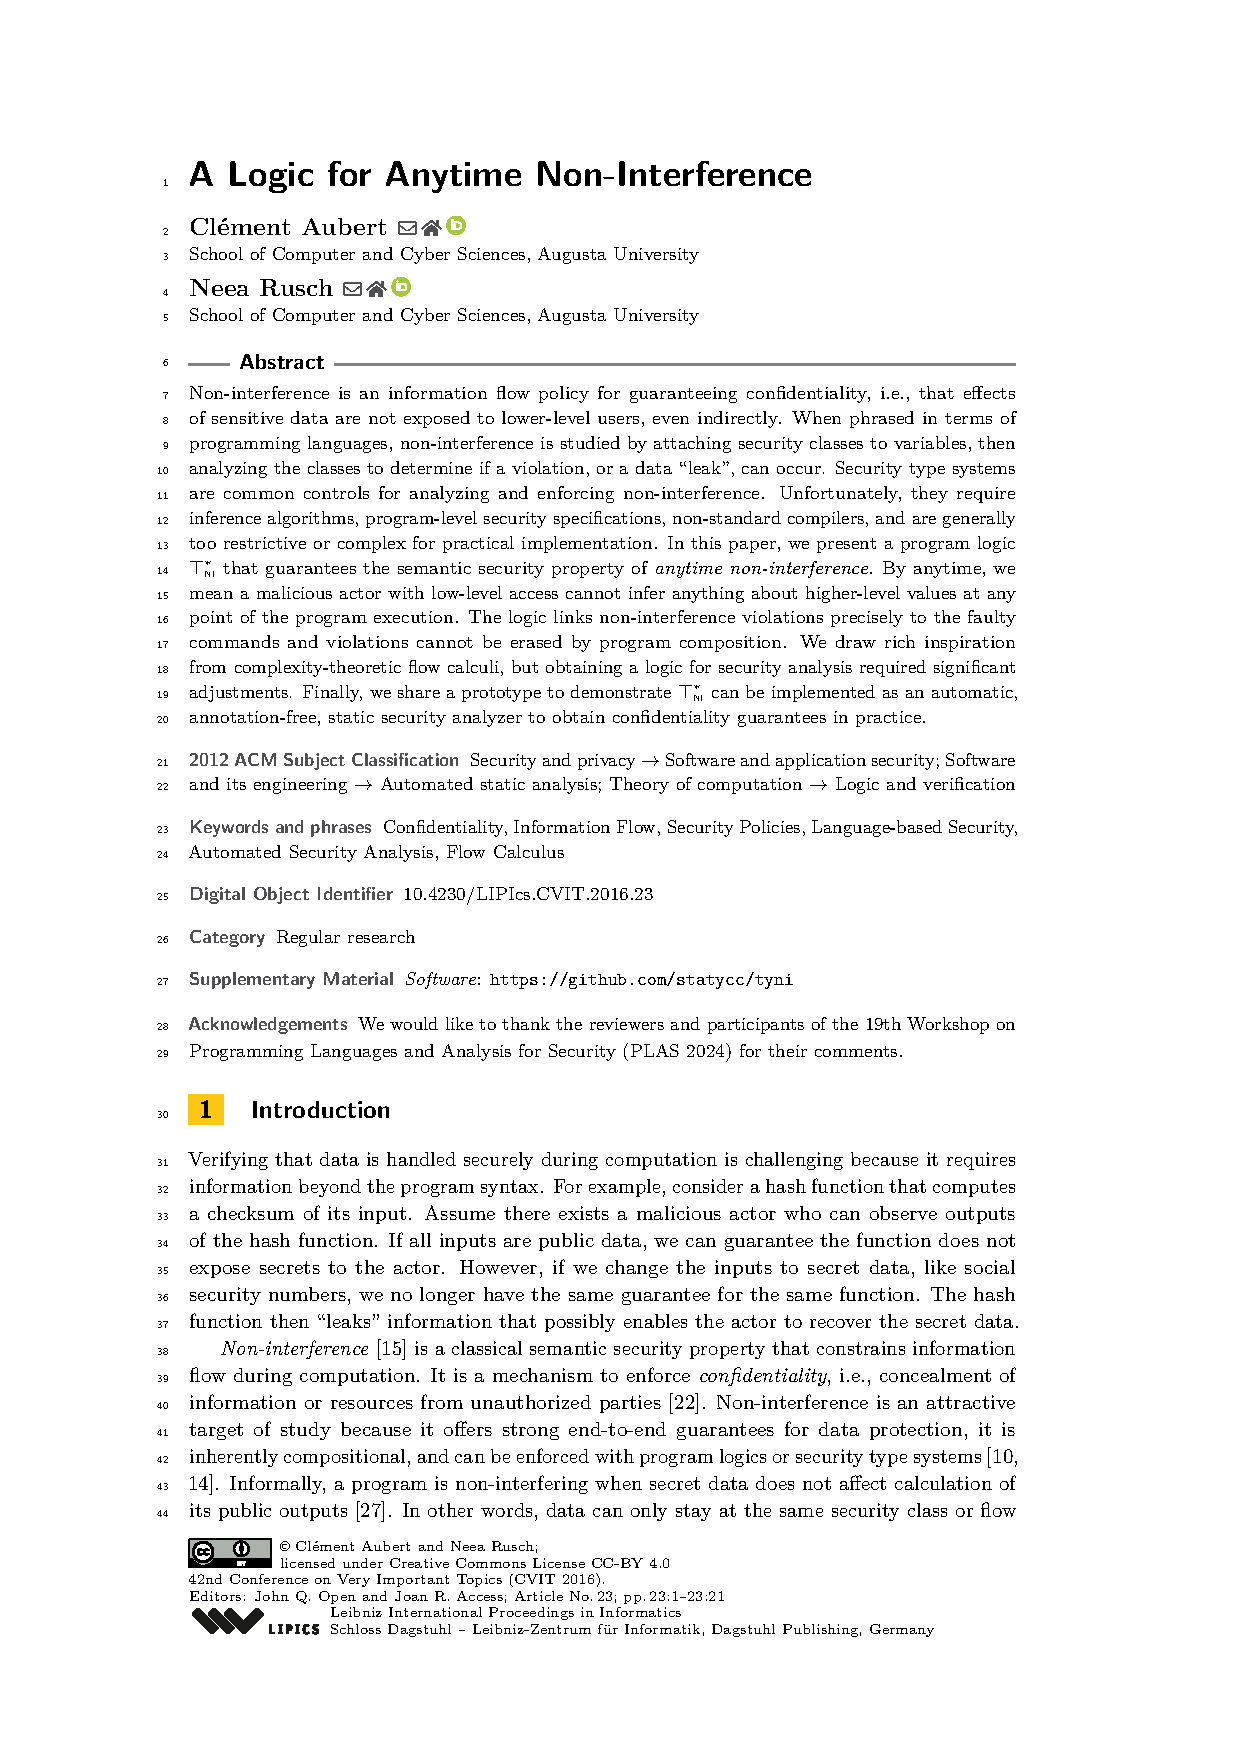
\includepdf[pages={1-},
    addtotoc={
        1,subsection,2,Introduction,sec:introduction,
        4,subsection,2,High-level Overview,sec:overview,
        4,subsection,2,The Non-interference Logic,ni-logic,
        9,subsection,2,Capturing Anytime Non-Interference,sec:at-soundness,
        10,subsection,2,Interpreting Function Calls in an Anytime Non-Interfering Context,sec:fct-calls,
        13,subsection,2,Practical Applications and Comparison,sec:apps,
        15,subsection,2,{Conclusion: Strengths, Limitations and Future Directions},sec:conclusion,
        18,subsection,2,{Appendix A: Proof of Thm. 16},sec:app-a,
        19,subsection,2,{Appendix B: Examples},sec:app-b},
    addtolist={
        5,figure,{A Simple Imperative while Language},fig:grammar,
        5,table,{Definition of Out, In and Occ for commands},table:ni-def-out-in-occ,
        7,figure,{Statement Examples, Sets, Representations of Possible Violation(s)},fig:ni-dependences,
        7,figure,{Security-Flow Matrix of Compositions},fig:ni-composition,
        12,figure,{Statement Examples, Interpretation and Sets -- Involving Effects},fig:fct-effect,
        18,lstlisting,{Assignment case},lst:ni-assign,
        18,lstlisting,{Loop case},lst:ni-loop,
        18,lstlisting,{Branching case},lst:ni-branch},
    pagecommand={\thispagestyle{empty}%
    \addtoindexm{Dependency Core Calculus}{15}
    \addtoindexm{Hasse diagram}{3,6,20}
    \addtoindexm{Polybench/C}{21}
    \addtoindexm{Rice's Theorem}{2}
    \addtoindexm{attacker (adversary)}{3,7,9,13}
    \addtoindexm{attacker model}{3}
    \addtoindexm{bytecode}{13,14}
    \addtoindexm{complexity class}{15}
    \addtoindexm{confidentiality}{1,14}
    \addtoindexm{declassification}{15}
    \addtoindexm{dependence analysis}{5,15}
    \addtoindexm{dynamic code loading}{2}
    \addtoindexm{empty matrix}{7}
    \addtoindexm{hollow matrix}{5,6,19}
    \addtoindexm{imperative programs}{3,4,15}
    \addtoindexm{information flow!control}{3}
    \addtoindexm{information flow!explicit}{2,4}
    \addtoindexm{information flow!implicit}{2,4,8,15}
    \addtoindexm{information flow!policy}{1,3,6,14,15,20,21}}
    \addtoindexm{information flow}{1,2,3,14,19,21}
    \addtoindexm{intermediate representation}{14}
    \addtoindexm{language-based security}{2,14,15}
    \addtoindexm{lattice}{3}
    \addtoindexm{monoid}{5,6,8}
    \addtoindexm{non-interference!anytime}{1,2,3,8,9,10,12,13,14,15,18,19,20,21}
    \addtoindexm{non-interference!progress-sensitive}{2}
    \addtoindexm{non-interference!termination-insensitive}{2}
    \addtoindexm{non-interference}{1,2,3,4,5,8,9,10,13,14,15,18,19}
    \addtoindexm{program centric attacker model}{3}
    \addtoindexm{security class}{1,2,3,4,5,6,7,8,9,10,11,13,14,15}
    \addtoindexm{security objective}{3}
    \addtoindexm{security type system}{1,15}
    \addtoindexm{security type}{3,15}
    \addtoindexm{security-flow matrix}{4,5,6,7,11,14,21}
    \addtoindexm{side effect}{2,3,10,12,13}
    \addtoindexm{system model}{3}
    \addtoindexm{termination}{2,9,14}
]{pdf/pubs_ni.2025.pdf}